\documentclass[border=1.5pt]{standalone}
\usepackage{amsmath,amssymb}
\usepackage{tikz}
\usetikzlibrary{arrows.meta,calc,positioning,shapes,shapes.misc,shapes.geometric,backgrounds,fit,decorations.pathreplacing,quantikz2}
% Shared colors and styles for the XYZ^2 figures.
% Pauli types: bright tones for fills and bands, deep (800) shades of the same hues for labels.
% The label shades keep the hue of each Pauli, are well separated from each other (CIEDE2000 > 20)
% and have a contrast ratio of at least 2.9 on the coral cells and 4.5 on the sunflower cells.
\definecolor{PauliX}{HTML}{F97316}
\definecolor{PauliY}{HTML}{EC4899}
\definecolor{PauliZ}{HTML}{9333EA}
\definecolor{PauliXText}{HTML}{AC340B}
\definecolor{PauliYText}{HTML}{9D174D}
\definecolor{PauliZText}{HTML}{5B21B6}
% Generator classes: S0 (class B, even links, coral) and gauge (class A, odd links, sunflower)
\definecolor{Szero}{HTML}{F0435E}
\definecolor{SzeroText}{HTML}{BE123C}
\definecolor{Gauge}{HTML}{F59E0B}
\definecolor{GaugeText}{HTML}{B45309}
\colorlet{GaugeGray}{Gauge}
\definecolor{ClassB}{HTML}{FF8A99}
\definecolor{ClassA}{HTML}{FFD23F}
% Logical operators (X-bar violet, Z-bar crimson), errors, ink
\definecolor{LogicalZ}{HTML}{E11D48}
\definecolor{LogicalGold}{HTML}{7C3AED}
\definecolor{ErrRed}{HTML}{1C1917}
\definecolor{InkDark}{HTML}{292524}
\definecolor{InkSoft}{HTML}{57534E}
% Labels drawn on top of colored cells
\colorlet{CellText}{InkDark}
% Noise channels
\definecolor{ErrFlip}{HTML}{EF4444}
\definecolor{Idle}{HTML}{EC4899}
\definecolor{TwoQ}{HTML}{7C3AED}
% Protocol steps
\definecolor{StepPrep}{HTML}{F97316}
\definecolor{StepMeas}{HTML}{D946EF}
\definecolor{StepDec}{HTML}{7C3AED}
\definecolor{StepRec}{HTML}{DB2777}
\tikzset{
  qb/.style={circle, draw=InkDark, line width=0.6pt, fill=white,
             minimum size=4.2mm, inner sep=0pt, font=\scriptsize},
  qbsmall/.style={circle, draw=InkDark, line width=0.5pt, fill=white,
             minimum size=2.6mm, inner sep=0pt},
  hexedge/.style={line width=0.65pt, draw=InkSoft},
  linkedge/.style={line width=1.6pt, draw=InkDark},
  bndedge/.style={line width=0.65pt, draw=InkSoft, densely dashed},
  plabel/.style={font=\scriptsize\bfseries, inner sep=1pt},
  panel/.style={font=\small\bfseries, anchor=north west},
}

\providecommand{\ket}[1]{\left|#1\right\rangle}

\begin{document}
\setlength{\tabcolsep}{0pt}
\begin{tabular}{@{}l@{\hspace{7mm}}l@{}}
\textbf{(a)} & \textbf{(b)}\\[-2pt]
\raisebox{-0.5\height}{%
\begin{quantikz}[row sep={0.95cm,between origins}, column sep=0.34cm]
\lstick{\footnotesize ancilla $\ket{0}$} & \gate[style={fill=PauliX!25, draw=PauliX, line width=0.7pt}]{H} \slice[style={draw=InkSoft, dash pattern=on 2pt off 1.5pt, line width=0.5pt}, label style={text=InkSoft}]{\scriptsize\bfseries 1} & \ctrl{1} \slice[style={draw=InkSoft, dash pattern=on 2pt off 1.5pt, line width=0.5pt}, label style={text=InkSoft}]{\scriptsize\bfseries 2} & \gate[style={fill=PauliX!25, draw=PauliX, line width=0.7pt}]{H} \slice[style={draw=InkSoft, dash pattern=on 2pt off 1.5pt, line width=0.5pt}, label style={text=InkSoft}]{\scriptsize\bfseries 3} & \meter[style={fill=PauliZ!20, draw=PauliZ, line width=0.7pt}]{} \slice[style={draw=InkSoft, dash pattern=on 2pt off 1.5pt, line width=0.5pt}, label style={text=InkSoft}]{\scriptsize\bfseries 4} & \setwiretype{c} & \setwiretype{n} \\
\lstick{\footnotesize data $\ket{\psi}$} & \qwbundle{n} & \gate[style={fill=ClassB!45, draw=Szero, line width=0.7pt}]{G} & & & \gate[style={fill=ClassA!45, draw=Gauge, line width=0.7pt}]{P^{\,s}} \wire[u][1]{c} & \rstick{\footnotesize $\Pi^{+}\ket{\psi}$}
\end{quantikz}}
&
\raisebox{-0.5\height}{%
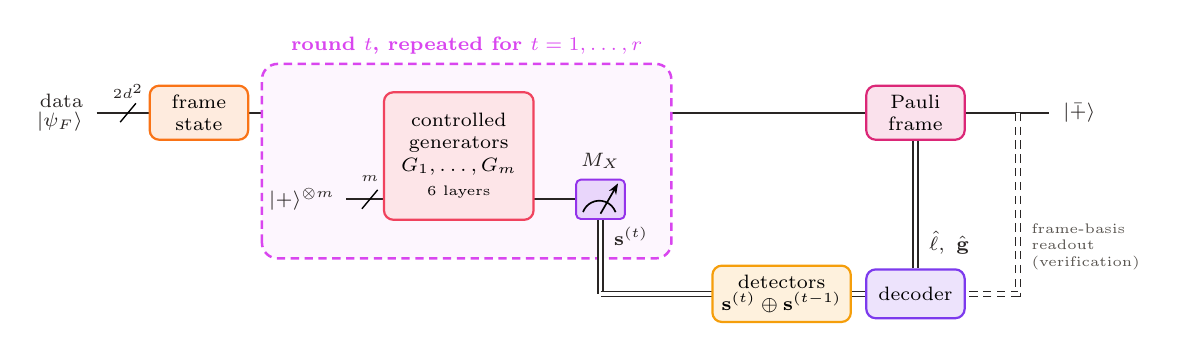
\begin{tikzpicture}[
  qw/.style={line width=0.8pt, draw=InkDark},
  cw/.style={draw=InkDark, line width=0.45pt, double, double distance=1.3pt},
  box/.style={draw=#1, fill=#1!14, line width=0.8pt, rounded corners=1.2mm, font=\scriptsize, align=center},
  lab/.style={font=\scriptsize, text=InkDark},
]
\def\yd{1.55} \def\ya{0.45} \def\yc{-0.75}
% ---------------- data wire
\node[lab, anchor=east, align=right] at (0,\yd) {data\\[-1pt] $\ket{\psi_F}$};
\draw[qw] (0.05,\yd) -- (12.15,\yd);
\draw[line width=0.5pt] (0.35,\yd-0.12) -- (0.55,\yd+0.12);
\node[font=\tiny, text=InkDark] at (0.45,\yd+0.27) {$2d^2$};
% frame preparation
\node[box=StepPrep, minimum width=1.25cm, minimum height=0.62cm] (F) at (1.35,\yd) {frame\\ state};
% ---------------- one extraction round (repeated r times)
\draw[densely dashed, draw=StepMeas, line width=0.9pt, rounded corners=2mm, fill=StepMeas!5] (2.15,\yc+0.45) rectangle (7.35,\yd+0.62);
\node[font=\scriptsize\bfseries, text=StepMeas, anchor=south] at (4.75,\yd+0.62) {round $t$, repeated for $t=1,\dots,r$};
\node[lab, anchor=east] at (3.2,\ya) {$\ket{+}^{\otimes m}$};
\draw[qw] (3.22,\ya) -- (6.15,\ya);
\draw[line width=0.5pt] (3.42,\ya-0.12) -- (3.62,\ya+0.12);
\node[font=\tiny, text=InkDark] at (3.52,\ya+0.27) {$m$};
\node[box=Szero, minimum width=1.9cm, minimum height=1.62cm] (C) at (4.65,{(\yd+\ya)/2})
  {controlled\\ generators\\ $G_1,\dots,G_m$\\[1pt] {\tiny 6 layers}};
\node[draw=PauliZ, fill=PauliZ!20, line width=0.7pt, minimum width=0.62cm, minimum height=0.5cm, rounded corners=0.6mm] (M) at (6.45,\ya) {};
\draw[line width=0.6pt] ($(M.south west)+(0.1,0.1)$) arc[start angle=160, end angle=20, radius=0.22];
\draw[-{Stealth[length=1.4mm]}, line width=0.6pt] ($(M.south)+(0,0.08)$) -- ($(M.north east)+(-0.1,-0.06)$);
\node[lab, anchor=south] at (M.north) {$M_X$};
\draw[cw] (M.south) -- (6.45,\yc);
\node[lab, anchor=west] at (6.5,-0.02) {$\mathbf{s}^{(t)}$};
% ---------------- classical processing
\draw[cw] (6.45,\yc) -- (7.95,\yc);
\node[box=Gauge, minimum width=1.55cm, minimum height=0.62cm] (Det) at (8.75,\yc) {detectors\\ $\mathbf{s}^{(t)}\oplus\mathbf{s}^{(t-1)}$};
\draw[cw] (Det.east) -- (9.85,\yc);
\node[box=StepDec, minimum width=1.25cm, minimum height=0.62cm] (Dec) at (10.45,\yc) {decoder};
\draw[cw] (Dec.north) -- (10.45,\yd-0.33);
\node[lab, anchor=west] at (10.5,{(\ya+\yc)/2+0.05}) {$\hat\ell,\ \hat{\mathbf{g}}$};
% ---------------- recovery and output
\node[box=StepRec, minimum width=1.25cm, minimum height=0.62cm] (R) at (10.45,\yd) {Pauli\\ frame};
\node[lab, anchor=west] at (12.2,\yd) {$\ket{\bar{+}}$};
% optional verification readout
\draw[cw, densely dashed] (11.75,\yd) -- (11.75,\yc) -- (Dec.east);
\node[lab, anchor=west, align=left, text=InkSoft] at (11.8,{(\ya+\yc)/2}) {\tiny frame-basis\\[-2pt] \tiny readout\\[-2pt] \tiny (verification)};
\end{tikzpicture}}
\end{tabular}

\end{document}
